\documentclass{article}
\usepackage[T1]{fontenc}
\usepackage{lmodern}
\usepackage{graphicx}
\usepackage{amsmath,amssymb}
\usepackage[a4paper,margin=2cm]{geometry}
\usepackage[absolute,overlay]{textpos}
\setlength{\TPHorizModule}{1mm}
\setlength{\TPVertModule}{1mm}
\usepackage[indonesian]{babel}
\usepackage{hyperref}
\setlength{\emergencystretch}{2em}
% unit: Halaman 16

\begin{document}

% === Halaman 16 (llm) ===

\section*{Visual Attack}

\begin{itemize}
    \item Memanfaatkan indera penglihatan $\rightarrow$ inspeksi kerusakan pada gambar akibat penyisipan
    \item Ide dasar :
\end{itemize}

\vspace{10mm}

% deskripsi: Diagram alir proses Visual Attack yang terdiri dari tiga kotak proses: 'media pembawa/ steganogram diserang' mengarah ke 'ekstraksi bit-bit yang berpotensi menjadi bit Pesan', yang kemudian mengarah ke 'Ilustrasi visual dari bit-bit yang telah diekstraksi dengan posisi yang sesuai dengan pixel sumbernya'.
% bbox normalisasi: [0.1980, 0.5510, 0.7610, 0.8760]
\begin{textblock*}{118.23mm}(41.58mm,163.65mm)
\noindent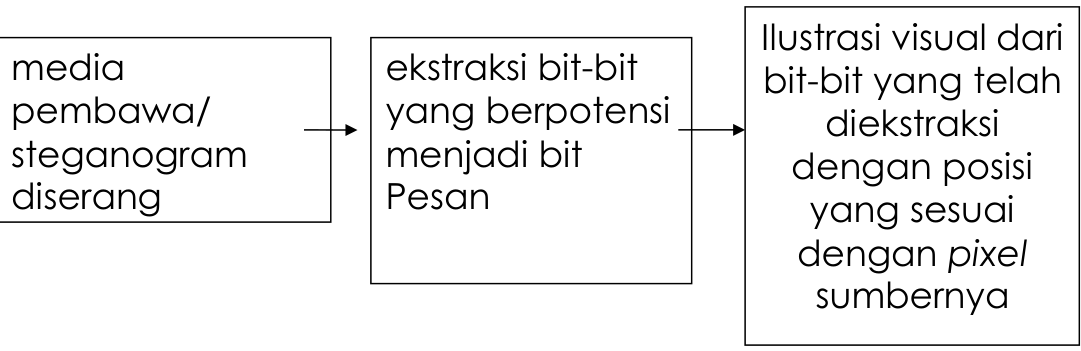
\includegraphics[width=118.23mm,height=96.52mm]{../../images/llm/page_016_img_01.png}%
\end{textblock*}

\end{document}
